\begin{frame}[fragile]{Tutorial: Priming}

\begin{columns}

\begin{column}{4.5cm}

\begin{onlyenv}<1->
\begin{lstlisting}[language=JuliaLocal, style=julia, basicstyle=\small]
i = Index(2)
j = Index(2)

i == j
\end{lstlisting}
\end{onlyenv}

\begin{onlyenv}<3->
\begin{lstlisting}[language=JuliaLocal, style=julia, basicstyle=\small]
i = Index(2)

prime(i)
i'
i == i'
noprime(i')
\end{lstlisting}
\end{onlyenv}

\end{column}

\begin{column}{4.5cm}

\begin{onlyenv}<1-1>
(dim=2|id=837) \\
(dim=2|id=899) \\
~\\
false \\
\end{onlyenv}

\begin{onlyenv}<2->

\includegraphics[width=0.8\textwidth]{
  slides/assets/i_neq_j.png
}
\vspace*{1.0cm}
\end{onlyenv}

\begin{onlyenv}<3-3>
(dim=2|id=837) \\
~\\
(dim=2|id=837)' \\
(dim=2|id=837)' \\
false \\
(dim=2|id=837)
\end{onlyenv}

\begin{onlyenv}<4->
\begin{center}

\includegraphics[width=0.2\textwidth]{
  slides/assets/i.png
} \\
\vspace*{0.5cm}
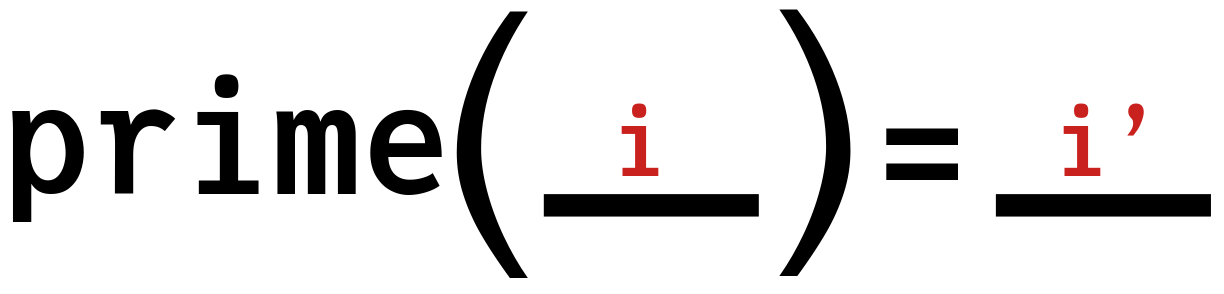
\includegraphics[width=1.0\textwidth]{
  slides/assets/prime_i.png
} \\

\includegraphics[width=0.7\textwidth]{
  slides/assets/i_neq_ip.png
}
\end{center}
\end{onlyenv}

\end{column}

\end{columns}

\end{frame}
